\section{Related Approaches}
\begin{frame}{Related Approaches}
  \begin{itemize}
    \item Optimization
      \begin{itemize}
        \item Deterministic
        \item Stochastic
      \end{itemize}
      \vspace*{14pt}
    \item Properties
      \begin{itemize}
        \item Stability
        \item Robustness
      \end{itemize}
      \vspace*{14pt}
    \item Utilizing global information
      \begin{itemize}
        \item Estimation of Distribution Algorithm (EDA)
        \item Model building
      \end{itemize}
  \end{itemize}
\end{frame}

\subsection{Real-coded Extended Compact Genetic Algorithm}


\begin{frame}{Discretization} 
  \begin{itemize} 
    \item Continuous domain $\rightarrow$ Discrete domain 
    \item Finding good solutions $\rightarrow$ Finding promising
      regions
    \item 2 traditional discretization methods
      \begin{itemize}
        \item Fixed-Height Histogram (FHH)
        \item Fixed-Width Histogram (FWH)
      \end{itemize}
      \vspace*{2pt}
  \end{itemize}
  \begin{minipage}{.45\textwidth}
    \begin{figure}
      \centering
      \includegraphics[bb = 144 82 686 502, clip, width =0.9\textwidth]{FHH.eps}
      \caption{FHH}
    \end{figure}
  \end{minipage}
  \begin{minipage}{.45\textwidth}
    \begin{figure}
      \centering
      \includegraphics[bb = 144 82 686 502, clip, width =0.9\textwidth]{FWH.eps}
      \caption{FWH}
    \end{figure}
  \end{minipage}

\end{frame}

\begin{frame}{Split on Demand}
  \begin{itemize}
    \item Solutions in each bin should not exceed $\gamma N$.
      \begin{itemize}
        \item $N$ is the population size.
        \item $\gamma$ defines the rate of one region.
      \end{itemize}
    \item $\gamma$ decays with a factor $\epsilon$.
  \end{itemize}
  \begin{figure}[h]
    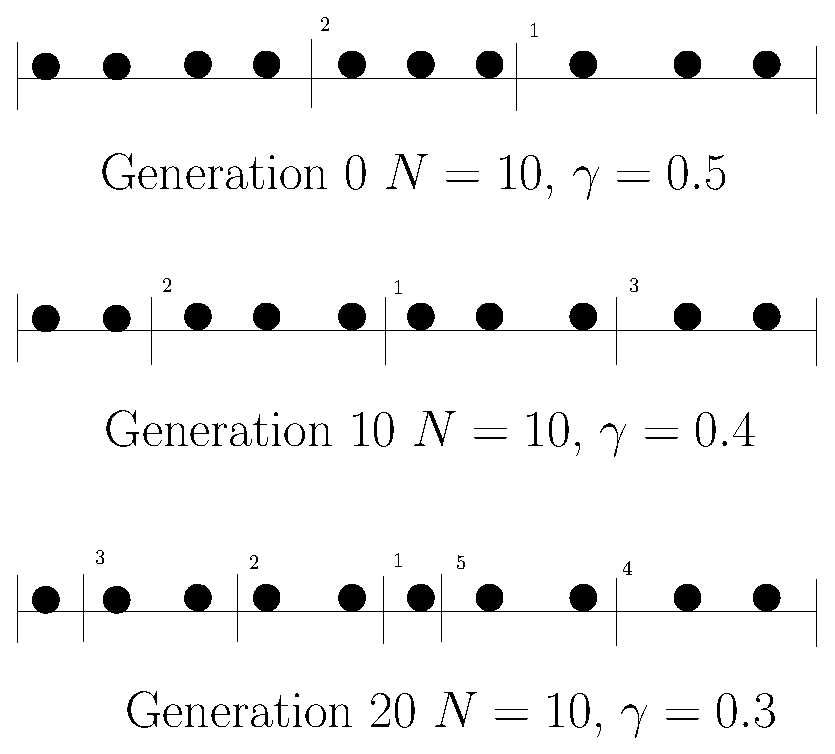
\includegraphics[bb = 100 86 635 502, clip, scale = 0.3]{SoD.eps}
    \caption{SoD}
  \end{figure}
\end{frame}

%\begin{frame}{EDA}
%  \begin{columns}
%    \begin{column}{.5\textwidth}
%      \begin{itemize}
%        \item Sometimes known as Probabilistic Model Building GA (PMBGA).
%          \begin{itemize}
%            \item Building model explicitly.
%            \item Linkage between decision variables are provided.
%          \end{itemize}
%          \vspace*{14pt}
%          \includegraphics[bb= 46 359 625 282, clip, width = 0.8\textwidth]{linkage}
%      %  \item  Extended Compact Genetic Algorithm (ECGA).
%      %    \begin{itemize}
%      %      \item Model is built according to population distribution.
%      %      \item Applying greedy search to refine model iteratively.
%      %    \end{itemize}
%      \end{itemize}
%    \end{column}
%    \begin{column}{.5\textwidth}
%      \begin{figure}[htp]
%        \centering
%        \includegraphics[width = 0.8\textwidth]{EDA.eps}
%      \end{figure}
%    \end{column}
%  \end{columns}
%\end{frame}

\begin{frame}{Extended Compact Genetic Algorithm}
  \begin{figure}
    \centering
  \includegraphics[bb = 1 125 900 450, clip, height = 0.35\textheight]{EDA2.eps}
\end{figure}
  \begin{figure}
    \centering
  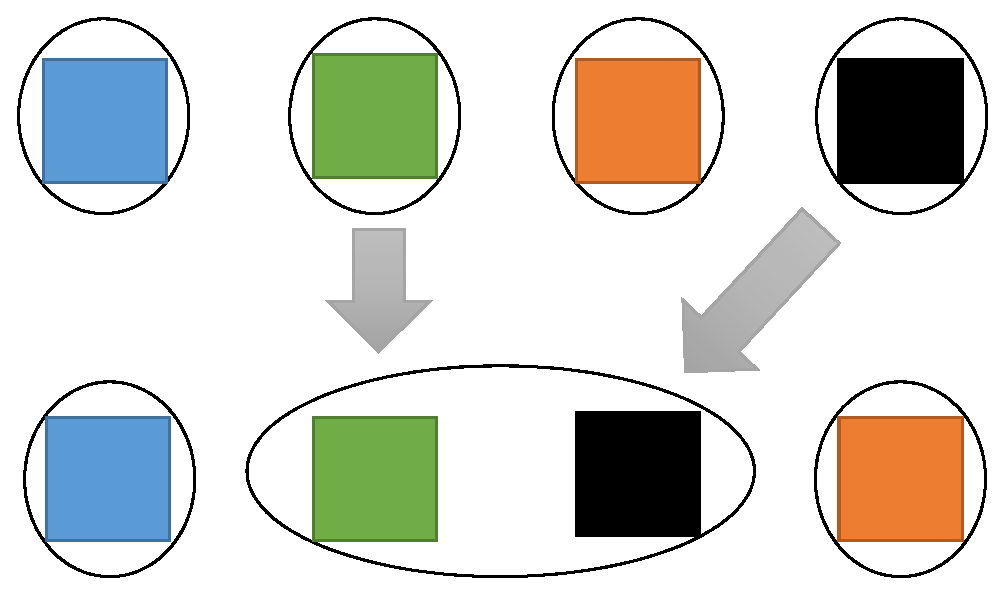
\includegraphics[bb = 32 150 552 450, clip, height = 0.15\textheight]{modelbuilding.eps}
\end{figure}
  \begin{itemize}
    \item $Pr(x_1,x_2,x_3,x_4) = Pr(x_1)Pr(x_2,x_4)Pr(x_3)$
  \end{itemize}
\end{frame}

\begin{frame}{Extended Compact Genetic Algorithm}
  \begin{figure}[t]  
    \includegraphics[bb = 50 73 777 554, clip, width=.8\textwidth]{ECGA.eps}
  \end{figure}
\end{frame}

\begin{frame}{Real-coded ECGA with SoD}
  \begin{figure}[t]  
    \includegraphics[bb = 50 73 777 554, clip, width=.8\textwidth]{rECGA.eps}
  \end{figure}

\end{frame}

\begin{frame}
  \frametitle{rECGA}
  \begin{itemize}
    \item Discretization 
      \begin{itemize}
        \item Continuous domain $\rightarrow$ Discrete domain $\rightarrow$
          Continuous domain
        \item Any distortion?
      \end{itemize}
  \end{itemize}
  \begin{figure}[htpb]
    \includegraphics[bb= 92 220 755 397, clip, width=0.5\textwidth]{Discretization.eps}
  \end{figure}
  \begin{itemize}
    \item Sampling
      \begin{itemize}
        \item Cliff between each bin is sometimes steep.
      \end{itemize}
      \begin{figure}[hpb]
        \includegraphics[bb = 67 21 774 546,clip, width = 0.3\textwidth]{Sampling.eps}
      \end{figure}
  \end{itemize}

\end{frame}


\begin{frame}{rECGA}
  \begin{itemize}
    \item rECGA tackles the difficulty of \alert{dimensionality}.
      \vspace*{14pt}
    \item Struggles in exploration, sampling.
      \vspace*{14pt}
    \item Why not solve continuous problem right in continuous domain?
  \end{itemize}
\end{frame}

\subsection{Covariance Matrix Adaptation Evolution Strategy}


\begin{frame}{Evolution Strategy (ES)}
  \begin{itemize}
    \item A search template for black-box optimization.
      \begin{itemize}
        \item Encoded in continuous domain.
      \end{itemize}
      \vspace*{14pt}
    \item New search points are generated based on current population.
      \vspace*{14pt}
    \item $x_i^{t+1} = m^t + \sigma N_i(0,C)$.
      \begin{itemize}
        \item $x_i^{t+1}$: $i$-th generated solution at generation $t+1$.
        \item $m^t$: weighted mean of population at generation $t$.
        \item $\sigma$: step size.
        \item $C$: Estimated distribution.
      \end{itemize}
  \end{itemize}
\end{frame}

\begin{frame}{Covariance Matrix Adaptation Evolution Strategy (CMA-ES)}
  \begin{itemize}
    \item A famous branch of ES
      \vspace*{14pt}
    \item Importance of $\sigma$ and $C$.
      \begin{itemize}
        \item Larger step size reinforces exploration while smaller
          reinforces exploitation.
          \begin{itemize}
            \item Choosing an fixed, appropriate number?
          \end{itemize}
        \item Covariance matrix determines the shape of estimated
          distribution.
          \begin{itemize}
            \item Determining the length of each axis.
            \item Representing the dependency among decision variables.
          \end{itemize}
      \end{itemize}
      \vspace*{14pt}
    \item CMA-ES features in the adoption of historical information.
      \begin{itemize}
        \item $\sigma$ and $C$ are adjusted accordingly.
      \end{itemize}
  \end{itemize}
\end{frame}

\begin{frame}{CMA-ES}
  \begin{figure}[t]
    \includegraphics[bb= 79 64 664 552, clip, width = 0.75\textwidth]{CMAES.eps}
  \end{figure}
\end{frame}

\begin{frame}{CMA-ES}
  \begin{itemize}
    \item An outstanding local optimizer
    \item Tackles \alert{non-separable} by maintaining a
      covariance matrix
    \item Usually encounters premature convergence
  \end{itemize}
  \begin{figure}[htpb]
    \centering
    \vfill\includegraphics[scale = 0.3]{LocalOptima.eps}
  \end{figure}
\end{frame}
%        \item Outer layer for exploration
%      \end{itemize}
%  \end{itemize}

%  \begin{columns}
%    \begin{column}{.33\textwidth}
%      \begin{figure}
%        \centering
%        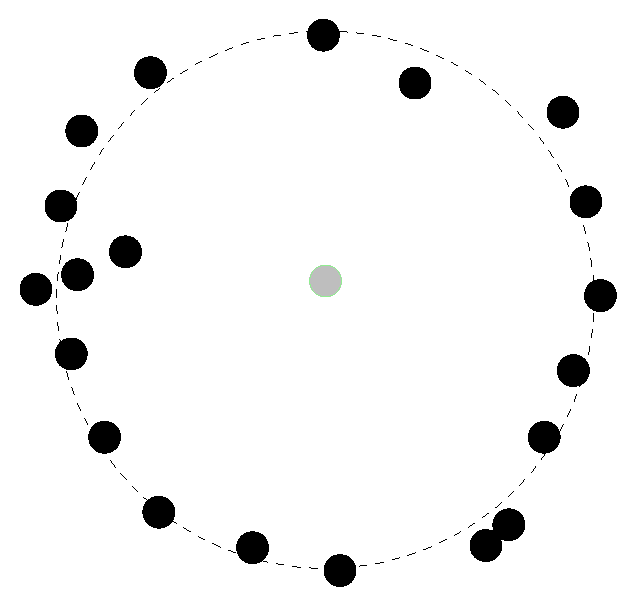
\includegraphics[width=.9\textwidth]{ES_0.eps}
%        \caption{$t$ = 0}
%      \end{figure}
%    \end{column}
%    \begin{column}{.33\textwidth}
%      \begin{figure}
%        \centering
%        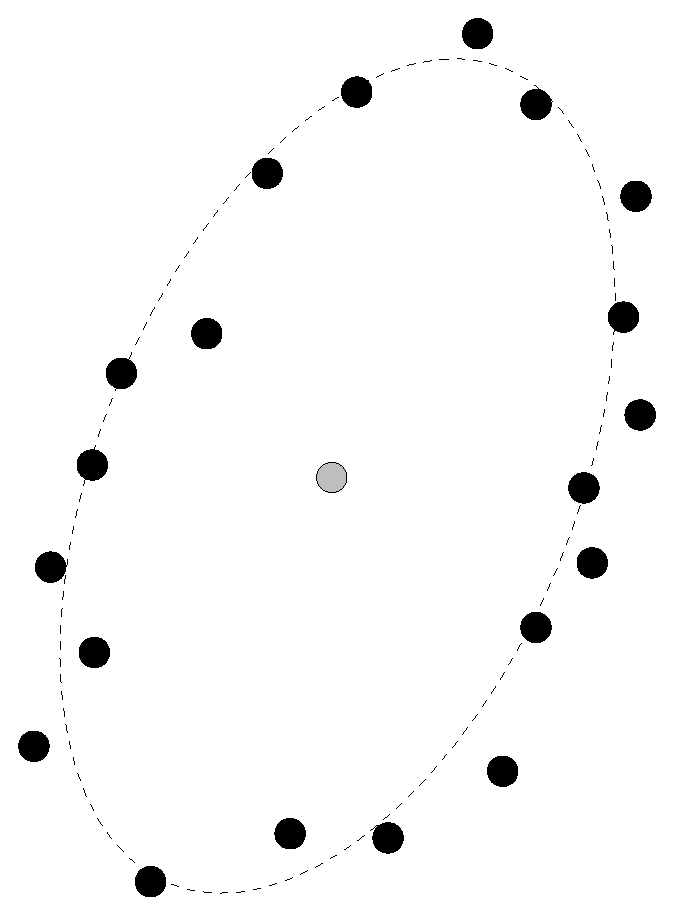
\includegraphics[width=.9\textwidth]{ES_10.eps}
%        \caption{$t$ = 10}
%      \end{figure}
%    \end{column}
%    \begin{column}{.33\textwidth}
%      \begin{figure}
%        \centering
%        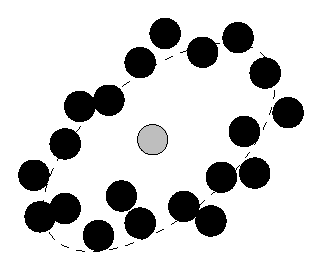
\includegraphics[width = .9\textwidth]{ES_20.eps}
%        \caption{$t$ = 20}
%      \end{figure}
%    \end{column}
%  \end{columns}

